\newpage
\subsection{Main PCB}
\label{subsec:main_pcb} 

In this section will be presented the work related to the design of the main PCB (printed circuit board), where the main electronics of the plush toy will be integrated.

\subsubsection{Features \& schematics}
\label{subsubsec:main_pcb/features&schematics} 

The first step, to begin with, was to allocate each electronic peripheral with the pins of the ESP-WROOM-32. Figure \ref{fig:pins_allocation} summarises the pin organisation in a table, where every peripheral corresponds to a colour. The "type" column shows if the pin is used for power ('P'), input ('I') or output ('O') signals. The pin number is indicated by the 'No.' column.

\begin{figure}[H]
    \centering
    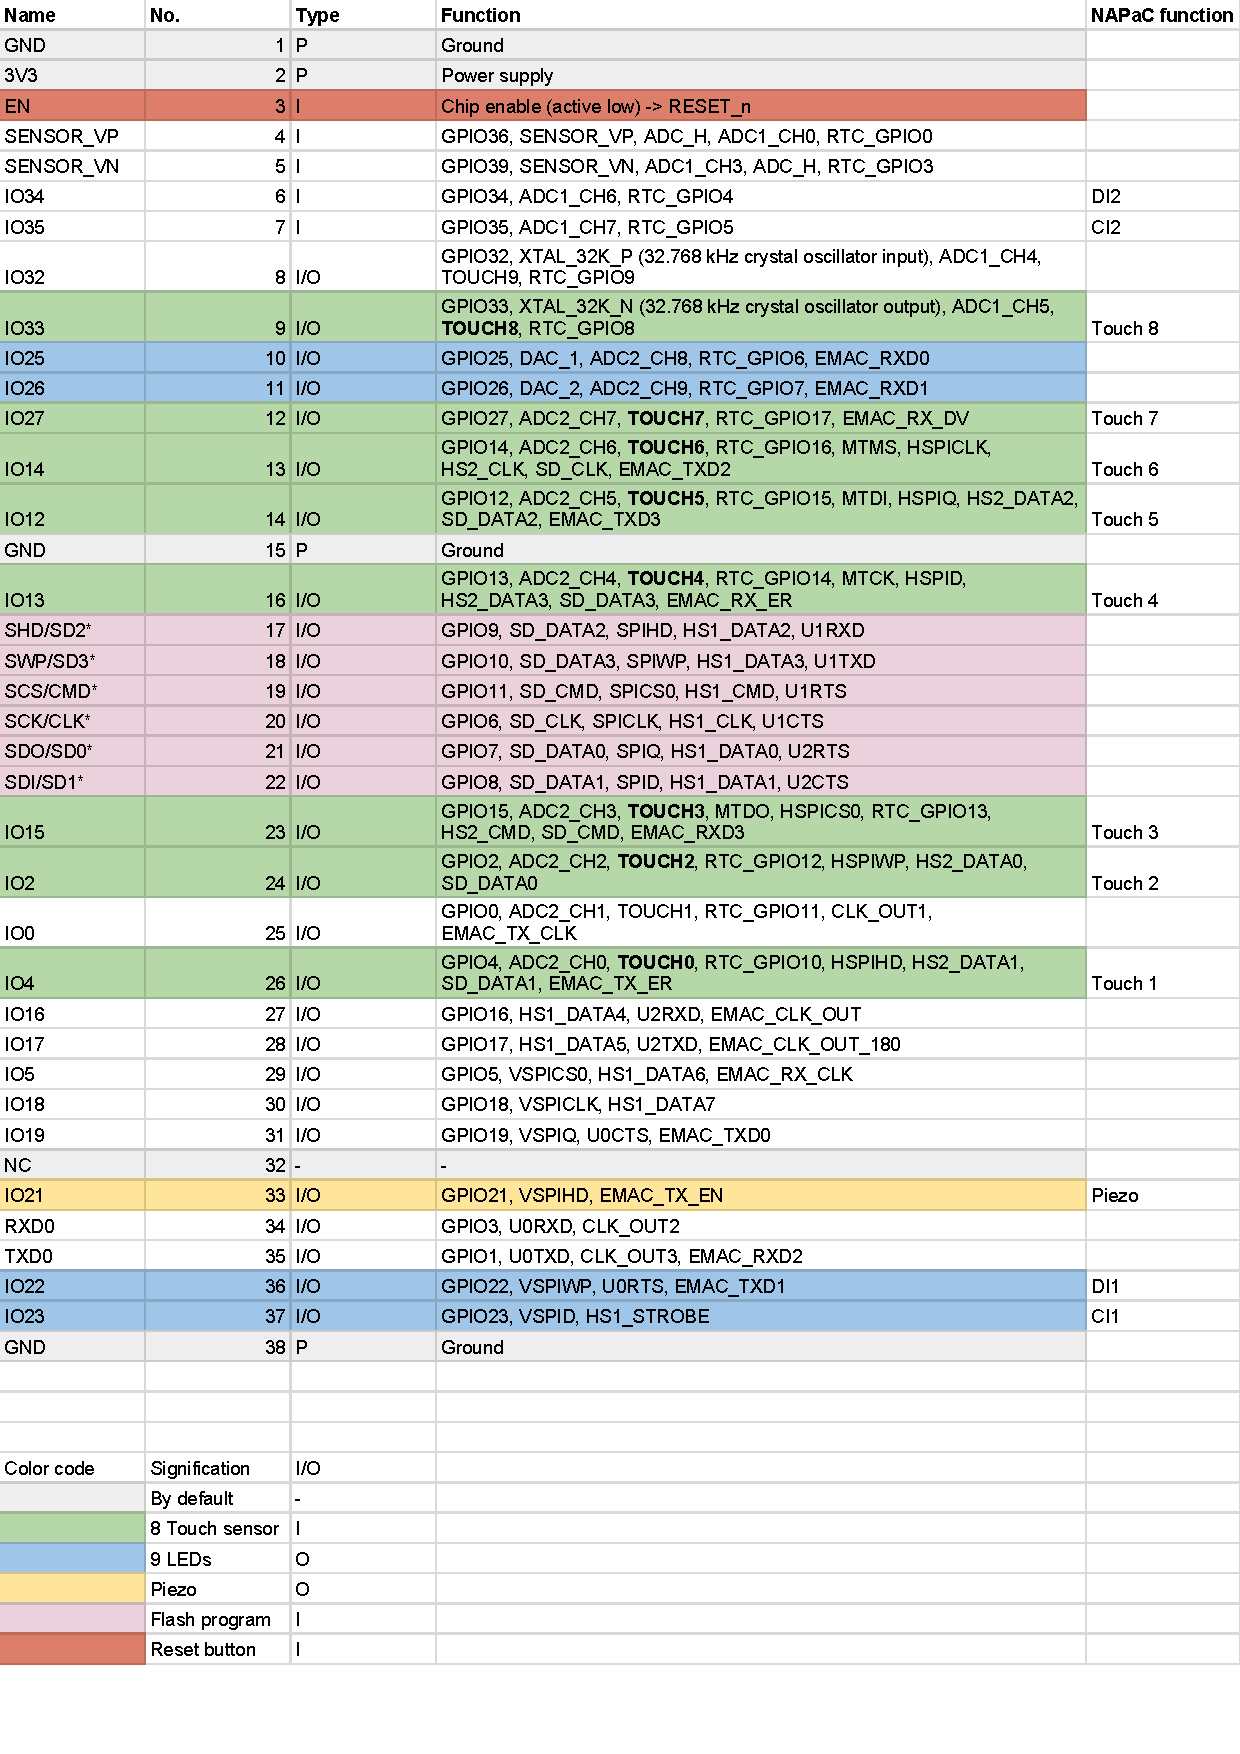
\includegraphics[width=0.72\textwidth]{images/EE_PinsallocationESPWROOM32-Sheet1.pdf}
    \caption{ESP-WROOM-32 pins allocation}
    \label{fig:pins_allocation}
\end{figure}

Once this work was done, the electronic schematic of the main PCB could be started. Based on the schematic of the ESP32-DevKitC (\cite{esp32devkitcschematic}), allowing existing functionality to be kept in the design of the main PCB. 

\medskip The main features of the design will be explored below.

\paragraph{ESP32 Module} As previously mentioned, the ESP-WROOM-32 is the main module of the main PCB, since the intelligence of the plush toy is stored on this component. C21 and C22 are decoupling capacitors, cancelling eventual small fluctuations of the input power (3V3).

\begin{figure}[H]
    \centering
    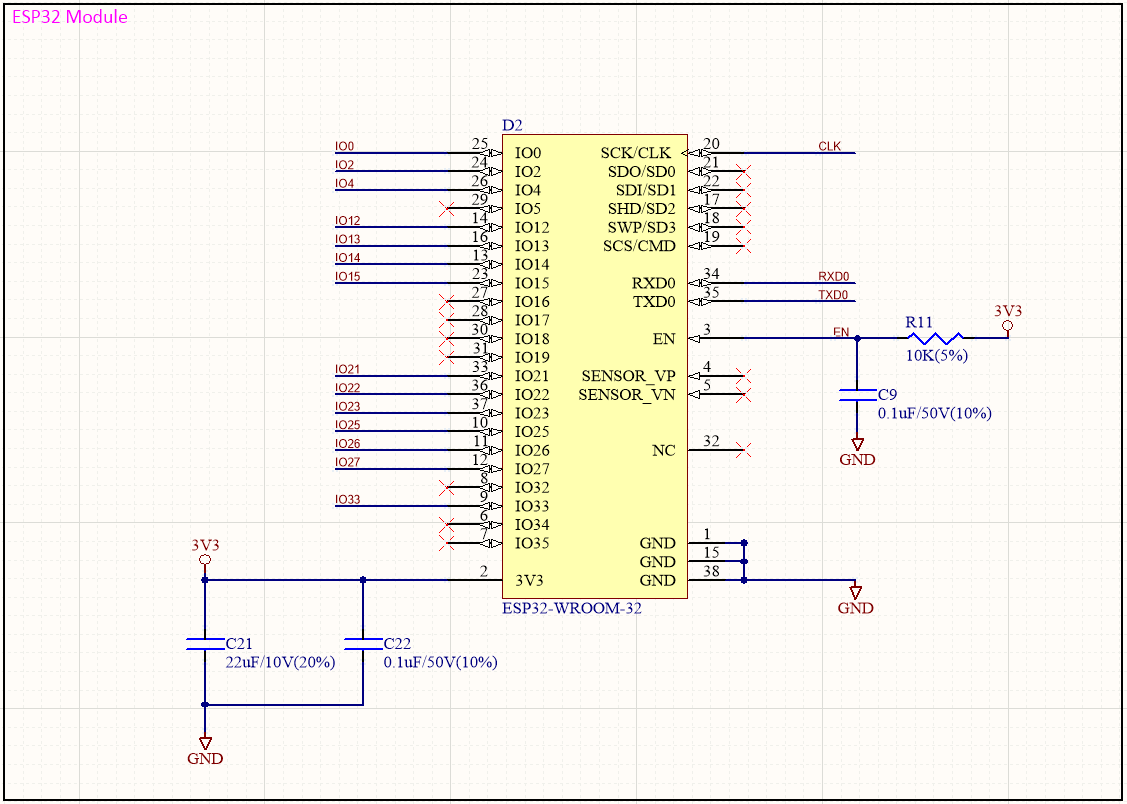
\includegraphics[width=0.9\textwidth]{images/EE_ESP32Module.PNG}
    \caption{ESP32 module schematic}
    \label{fig:ESP32_module_schematic}
\end{figure}

\paragraph{Power supply} As can be seen figure \ref{fig:power_supply_schematic}, two different constant voltages are needed in our electronic assembly. The LEDs APA102C require an input voltage of 5V, while the rest of the electronic components need 3V3. Therefore, the ACT4060A step down converter has been used, with 2A of output current (\cite{act4060adatasheet}) in order to supply enough power for all the 9 LEDs. On another hand, the LM1117 low-dropout linear regulator has been used to ensure a 3V3 voltage translation with 800 mA of output current (\cite{lm1117datasheet}), either from the 5V voltage coming from the micro-USB, or from the outputted voltage of the ACT4060A component.

\begin{figure}[H]
    \centering
    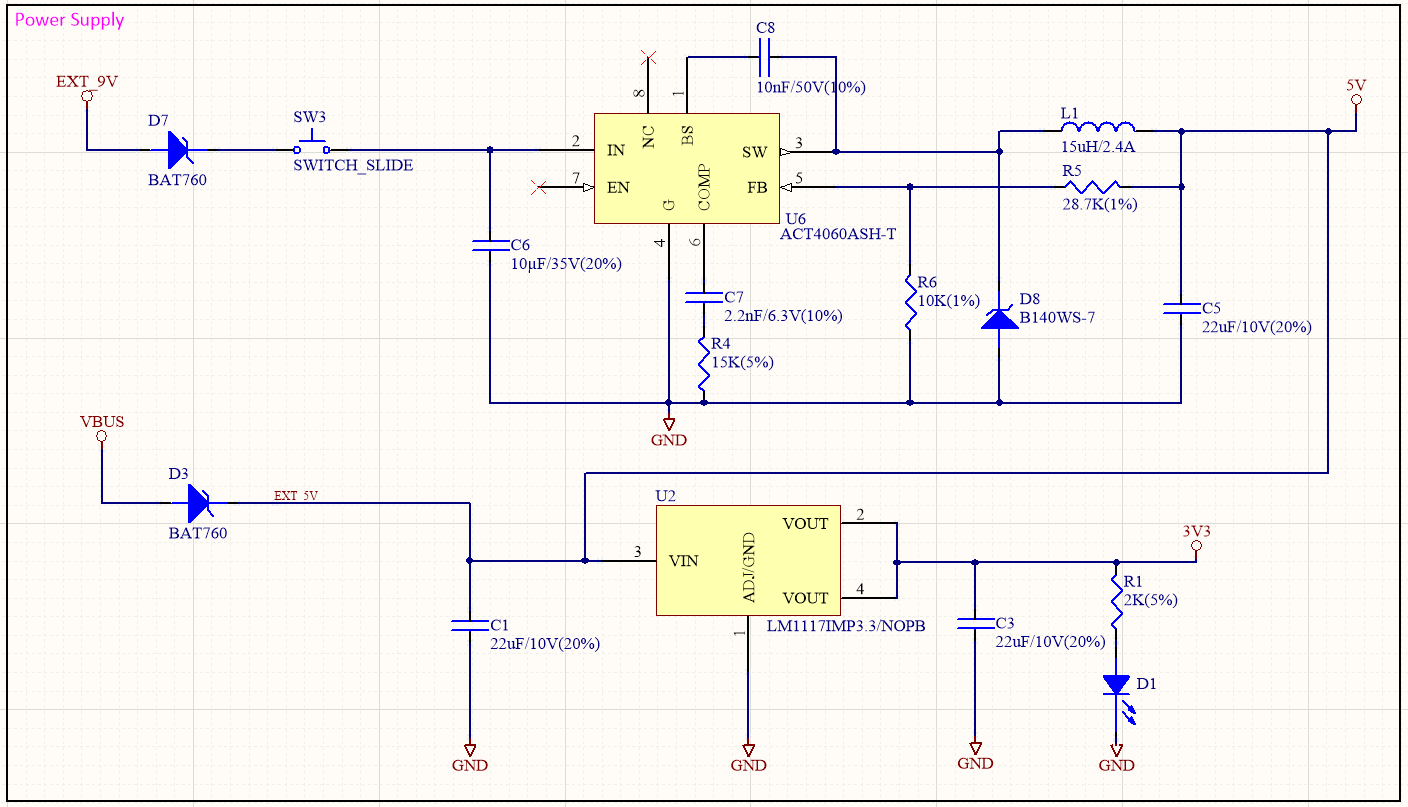
\includegraphics[width=0.9\textwidth]{images/EE_PowerSupply.PNG}
    \caption{Power supply schematic}
    \label{fig:power_supply_schematic}
\end{figure}


\paragraph{Micro USB \& USB-UART} The component on the top left corner of figure \ref{fig:MicroUSB&USB-UART_schematic} is the micro-USB connector. The two S8050-G-NPN transistor allow to program the microcontroller. Holding down the Boot button and pressing the EN button initiates the firmware download mode (refer to figure \ref{fig:SwitchButtons_schematic}). Then, the user can download firmware through the serial port. Finally, the CP2102N-GQFN24 component corresponds to the USB-to-UART bridge controller (\cite{cp2102datasheet}).

\begin{figure}[H]
    \centering
    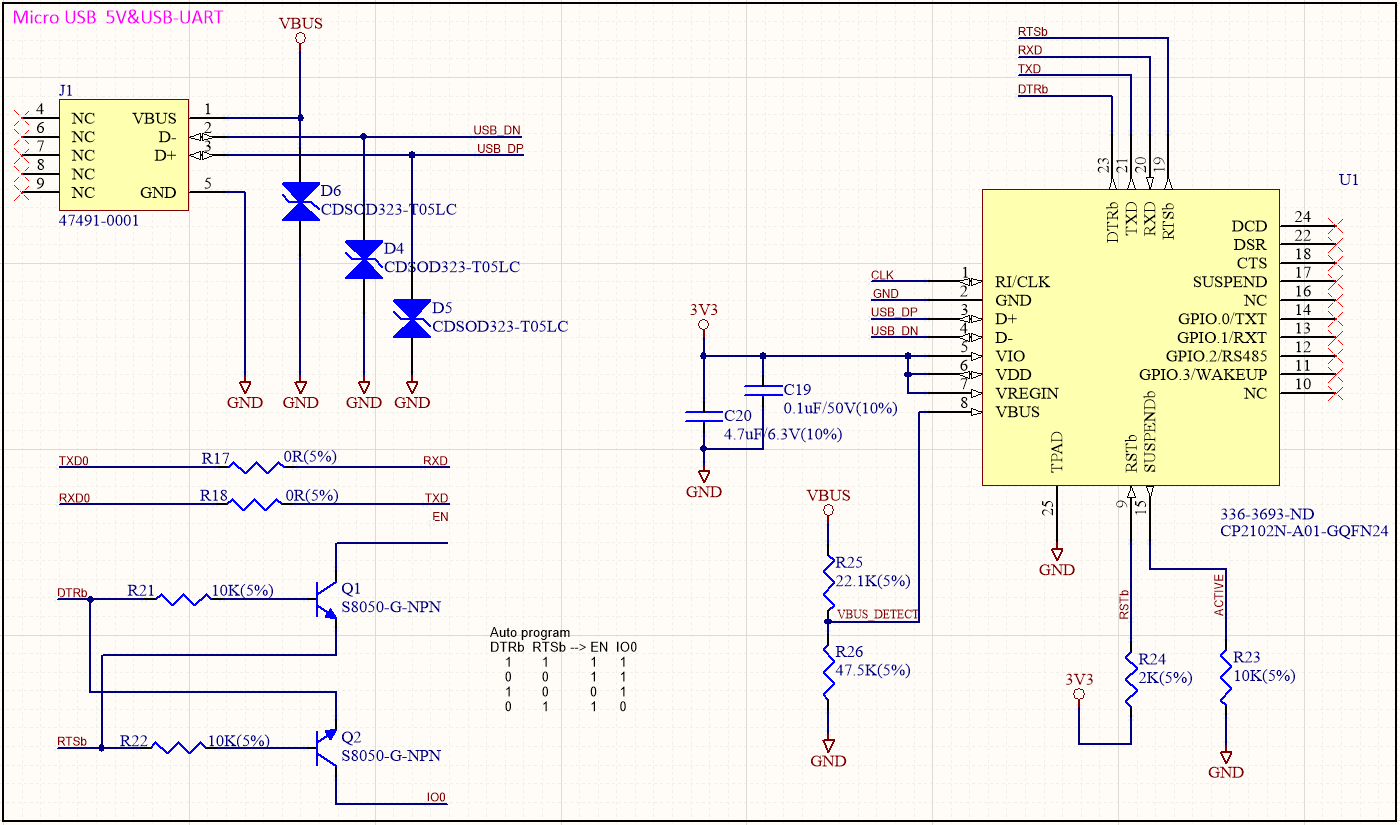
\includegraphics[width=0.9\textwidth]{images/EE_MicroUSB&USB-UART.PNG}
    \caption{Micro USB \& USB-UART schematic}
    \label{fig:MicroUSB&USB-UART_schematic}
\end{figure}

\paragraph{LEDs Voltage Translation} As already explained previously, the LEDs APA102C require an input voltage of 5V, also for the command signals. Therefore, two SN74LVC2T45 components, dual-bit and dual-supply bus transceiver with configurable voltage translation (\cite{sn74lvc2t45datasheet}), have been used to translate the voltage from the microcontroller at 3V3, to 5V.

\begin{figure}[H]
    \centering
    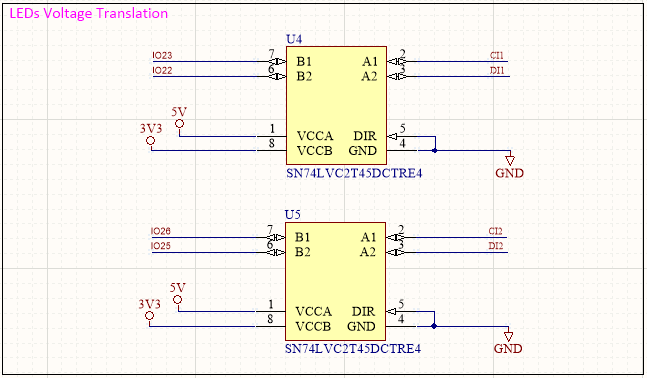
\includegraphics[width=0.9\textwidth]{images/EE_LEDsVoltageTranslation2.PNG}
    \caption{LEDs voltage translation schematic}
    \label{fig:LEDsVoltageTranslation_schematic}
\end{figure}


\paragraph{Switch Buttons} Two switch buttons PTS645 are used for the boot and the EN/reset of the microcontroller, as mentioned previously.

\begin{figure}[H]
    \centering
    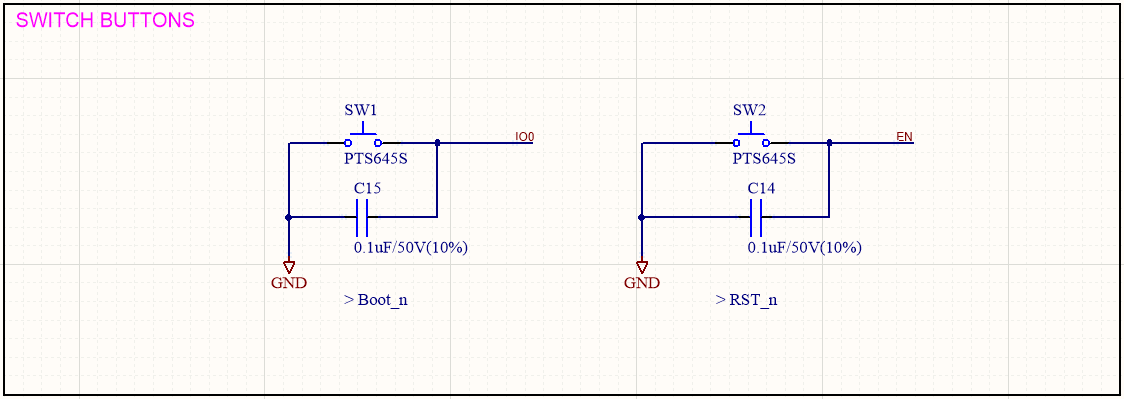
\includegraphics[width=0.9\textwidth]{images/EE_SwitchButtons.PNG}
    \caption{Switch buttons schematic}
    \label{fig:SwitchButtons_schematic}
\end{figure}


\paragraph{Connectors} Two connectors of 21 pins are interface the PCB with the battery supplying 9V power, the LED strip and the capacitive touch sensors. All the signals that have been doubled are here for debug purposes and design constraints. In fact, a wide pitch between two pins to be connected with textile wires was needed to prevent them intersecting each other, thus avoiding short circuits.

\begin{figure}[H]
    \centering
    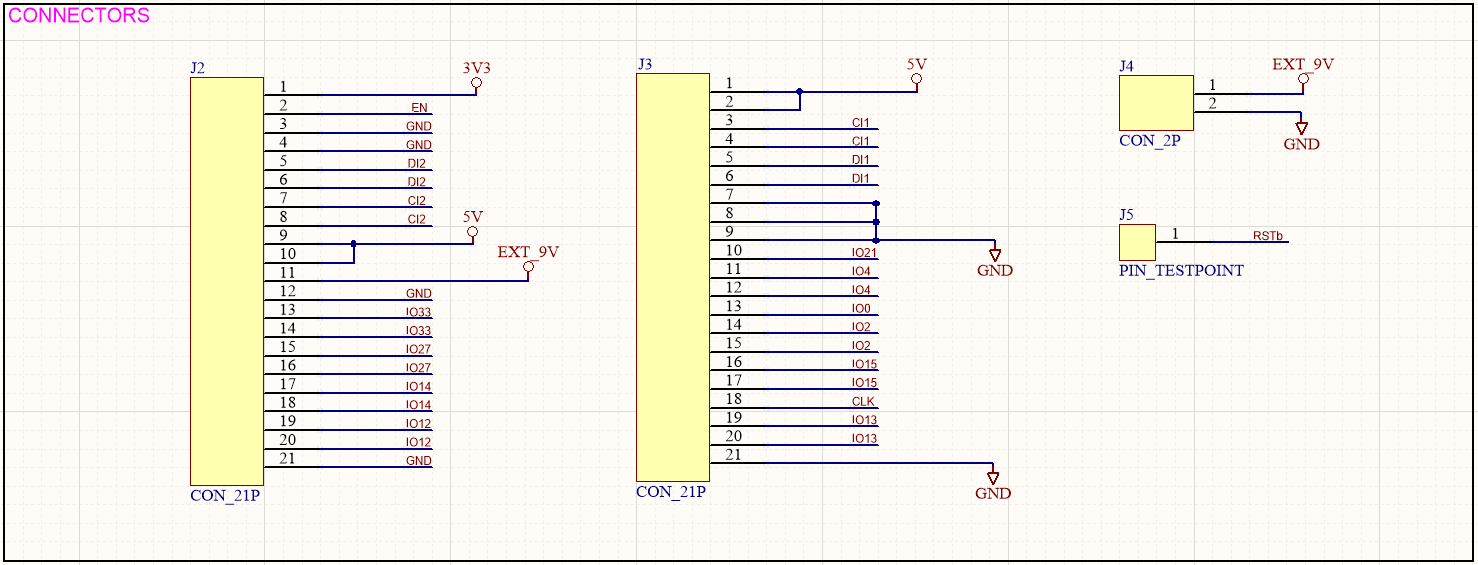
\includegraphics[width=0.9\textwidth]{images/EE_Connectors.PNG}
    \caption{Connectors schematic}
    \label{fig:connectors_schematic}
\end{figure}

The full schematic can be found in appendix, figure \ref{fig:main_pcb_schematic}.


\subsubsection{Bill of materials (BOM)}
\label{subsubsec:main_pcb/bill_of_materials} 

The resulting bill of materials is tabulated figure \ref{fig:BOM}. 

\begin{figure}[H]
    \centering
    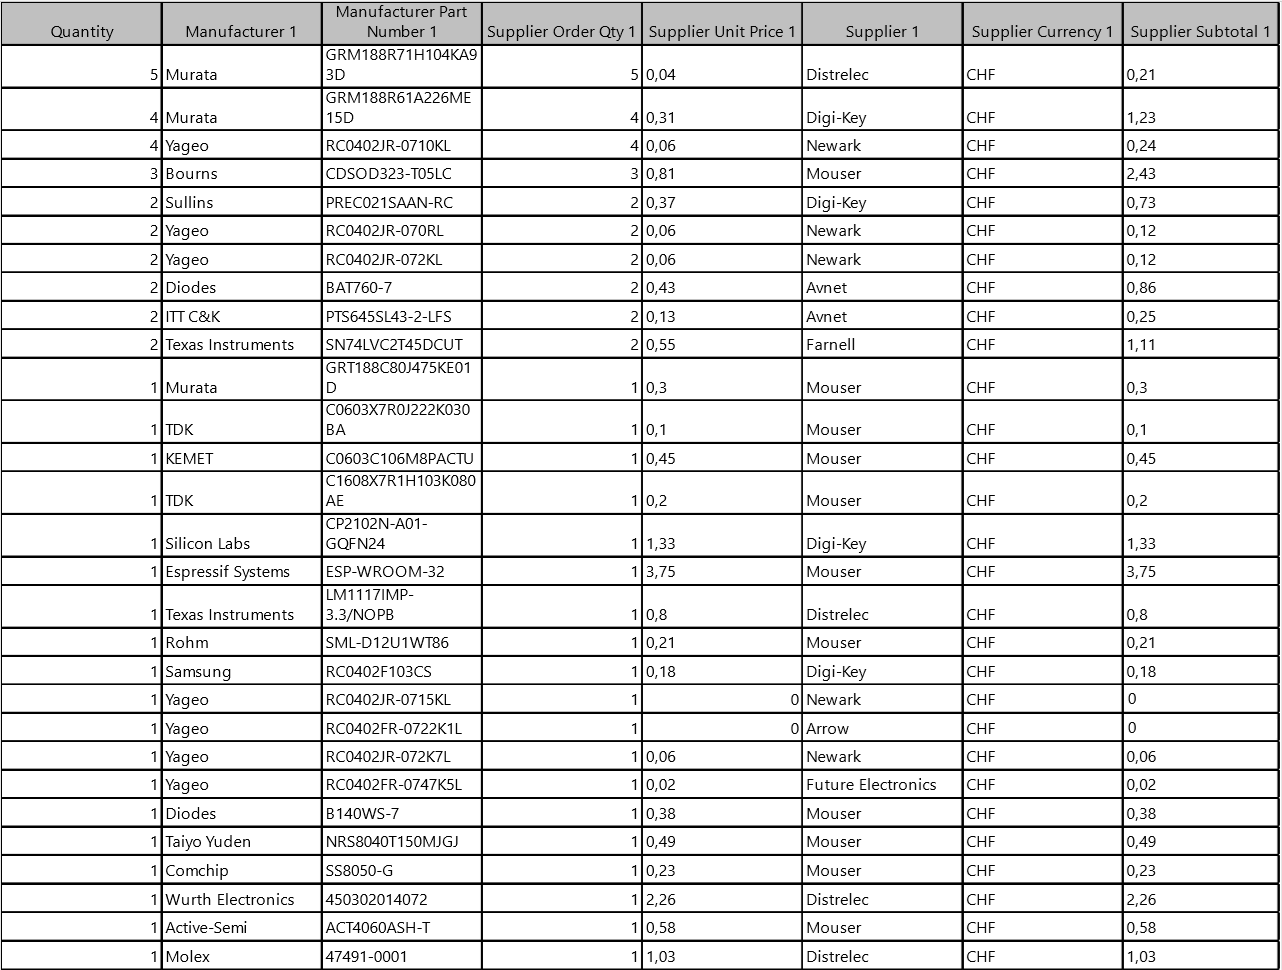
\includegraphics[width=0.9\textwidth]{images/EE_BOM.png}
    \caption{Electronic bill of materials}
    \label{fig:BOM}
\end{figure}

\subsubsection{Main PCB design}
\label{subsubsec:main_pcb/design} 


